\documentclass[12pt]{article}
\usepackage[utf8]{inputenc}
\usepackage{amsmath, amssymb}
\usepackage{geometry}
\usepackage{enumitem}
\usepackage{fancyhdr}
\usepackage{booktabs}
\usepackage{longtable}
\usepackage{array}
\usepackage{graphicx}
\usepackage{float}
\usepackage{hyperref}
\usepackage{listings}
\usepackage{xcolor}
\geometry{margin=1in}

\pagestyle{fancy}
\fancyhf{}
\renewcommand{\footrulewidth}{0.4pt}
\fancyfoot[R]{\thepage}

\setlength{\parindent}{0pt}
\setlength{\parskip}{0.3em}

% Improve line breaking
\sloppy

% Compact spacing for lists
\setlist{itemsep=1pt, topsep=2pt, parsep=0pt, leftmargin=3em}

% Code listing style
\lstset{
    basicstyle=\ttfamily\small,
    breaklines=true,
    frame=single,
    backgroundcolor=\color{gray!10}
}

\title{DBA5101: Portfolio Optimization Using Regularized Linear Regression}
\author{}
\date{}

\begin{document}

\begin{titlepage}
    \centering
    \vspace*{1cm}
    {\Huge\bfseries DBA5106 Group Project\\[0.5em]}
    {\Huge Portfolio Optimization Using Regularized Linear Regression \par}
    \vspace{1cm}
    
\includegraphics[width=0.30\textwidth]{nus_logo.png} \\[2em]
    {\large \textbf{Project Group 27}\par}
    \vspace{0.5cm}
    {\small
    WANG YING \\[0.2em]
    ZHAO QIYA \\[0.2em]
    ZHOU ZIHAN \\[0.2em]
    }
    \vspace{1cm}
    {\large
    National University of Singapore \\
    \vspace{0.5cm}
    Submission Date: \today \\
    \vspace{0.3cm}
    \href{https://github.com/ying-jeanne/Business_Analytics/tree/main/I}{Link to code repository}
    }
    \vfill
\end{titlepage}

\newpage

\section{Executive Summary}

This report presents a comprehensive analysis of portfolio optimization using regularized linear regression techniques to address overfitting issues inherent in minimum variance portfolios. We transform the traditional minimizing risks portfolio optimization problem into a linear regression framework and apply LASSO and Ridge regularization, with additional data transformation improvements for enhanced performance.

Using daily returns data from 100 portfolios formed on Market Equity (ME) and Operating Profitability (OP) from 1963 to 2025, we implement multiple approaches: baseline 126-day windows, extended 252-day windows, and 9-portfolio grouping (3×3 ME/OP matrix). Our analysis demonstrates that data transformation techniques significantly improve performance beyond regularization alone.

\textbf{Key Findings:}
\begin{itemize}
    \item LASSO regression provides sparse portfolio solutions with feature selection
    \item Ridge regression offers effective shrinkage to reduce parameter estimation noise
    \item Extended 252-day windows improve all strategies through more data points
    \item Portfolio grouping (100→9) dramatically improves performance: LASSO (0.0710 Sharpe), Ridge (0.0660 Sharpe)
    \item Data transformation addresses overfitting more effectively than regularization alone
    \item Equal-weighted remains a robust benchmark across all approaches
\end{itemize}

\section{Introduction and Data}

\subsection{Problem Statement}
We address the portfolio optimization challenge where accurate return estimation is notoriously difficult (achieving 2\% test $R^2$ is considered strong performance in finance vs 90\% in other domains). Given this limitation, we focus on minimum variance portfolios but face overfitting issues with 100 portfolios and 126-day rolling windows. We transform this into a linear regression framework and apply LASSO and Ridge regularization to mitigate overfitting.

\subsection{Data Overview}
We use the "100 Portfolios ME/OP 10x10" dataset from CRSP (202507), specifically extracting the equal-weighted returns section (rows 15,651 to 31,278 in the CSV file) spanning July 1963 to June 2025.

\textbf{Data Preprocessing:}
\begin{itemize}
    \item \textbf{Date Conversion:} date converted to datetime objects
    \item \textbf{Missing Value Treatment:} Sentinel values (-99.99, -999) replaced with NaN and dropped eventually
    \item \textbf{Final Dataset:} Approximately 15,625 clean observations across 100 portfolios
\end{itemize}

\section{Results and Analysis}

\subsection{Portfolio Performance Comparison}
The performance analysis focuses on the validation period (January 2 to June 30, 2025) containing 122 trading days to provide unbiased out-of-sample evaluation. Our analysis reveals significant performance differences across portfolio strategies, with regularization techniques demonstrating superior risk-adjusted returns.

\textbf{Reproduction:}
To reproduce the baseline portfolio performance results presented in Table \ref{tab:performance}, run:
\begin{lstlisting}
python portfolio.py --mode 1
\end{lstlisting}

\begin{table}[H]
\centering
\caption{Portfolio Performance Metrics (Validation Period: 2025-01-02 to 2025-06-30)}
\label{tab:performance}
\begin{tabular}{lccc}
\toprule
Strategy & Daily Mean Return (\%) & Daily Volatility (\%) & Sharpe Ratio \\
\midrule
EW & 2.70 & 163.65 & 0.0165 \\
MinVar & -17.88 & 135.80 & -0.1317 \\
LASSO & 4.30 & 97.44 & 0.0442 \\
Ridge & 4.12 & 94.61 & 0.0436 \\
\bottomrule
\end{tabular}
\end{table}

\begin{figure}[H]
\centering
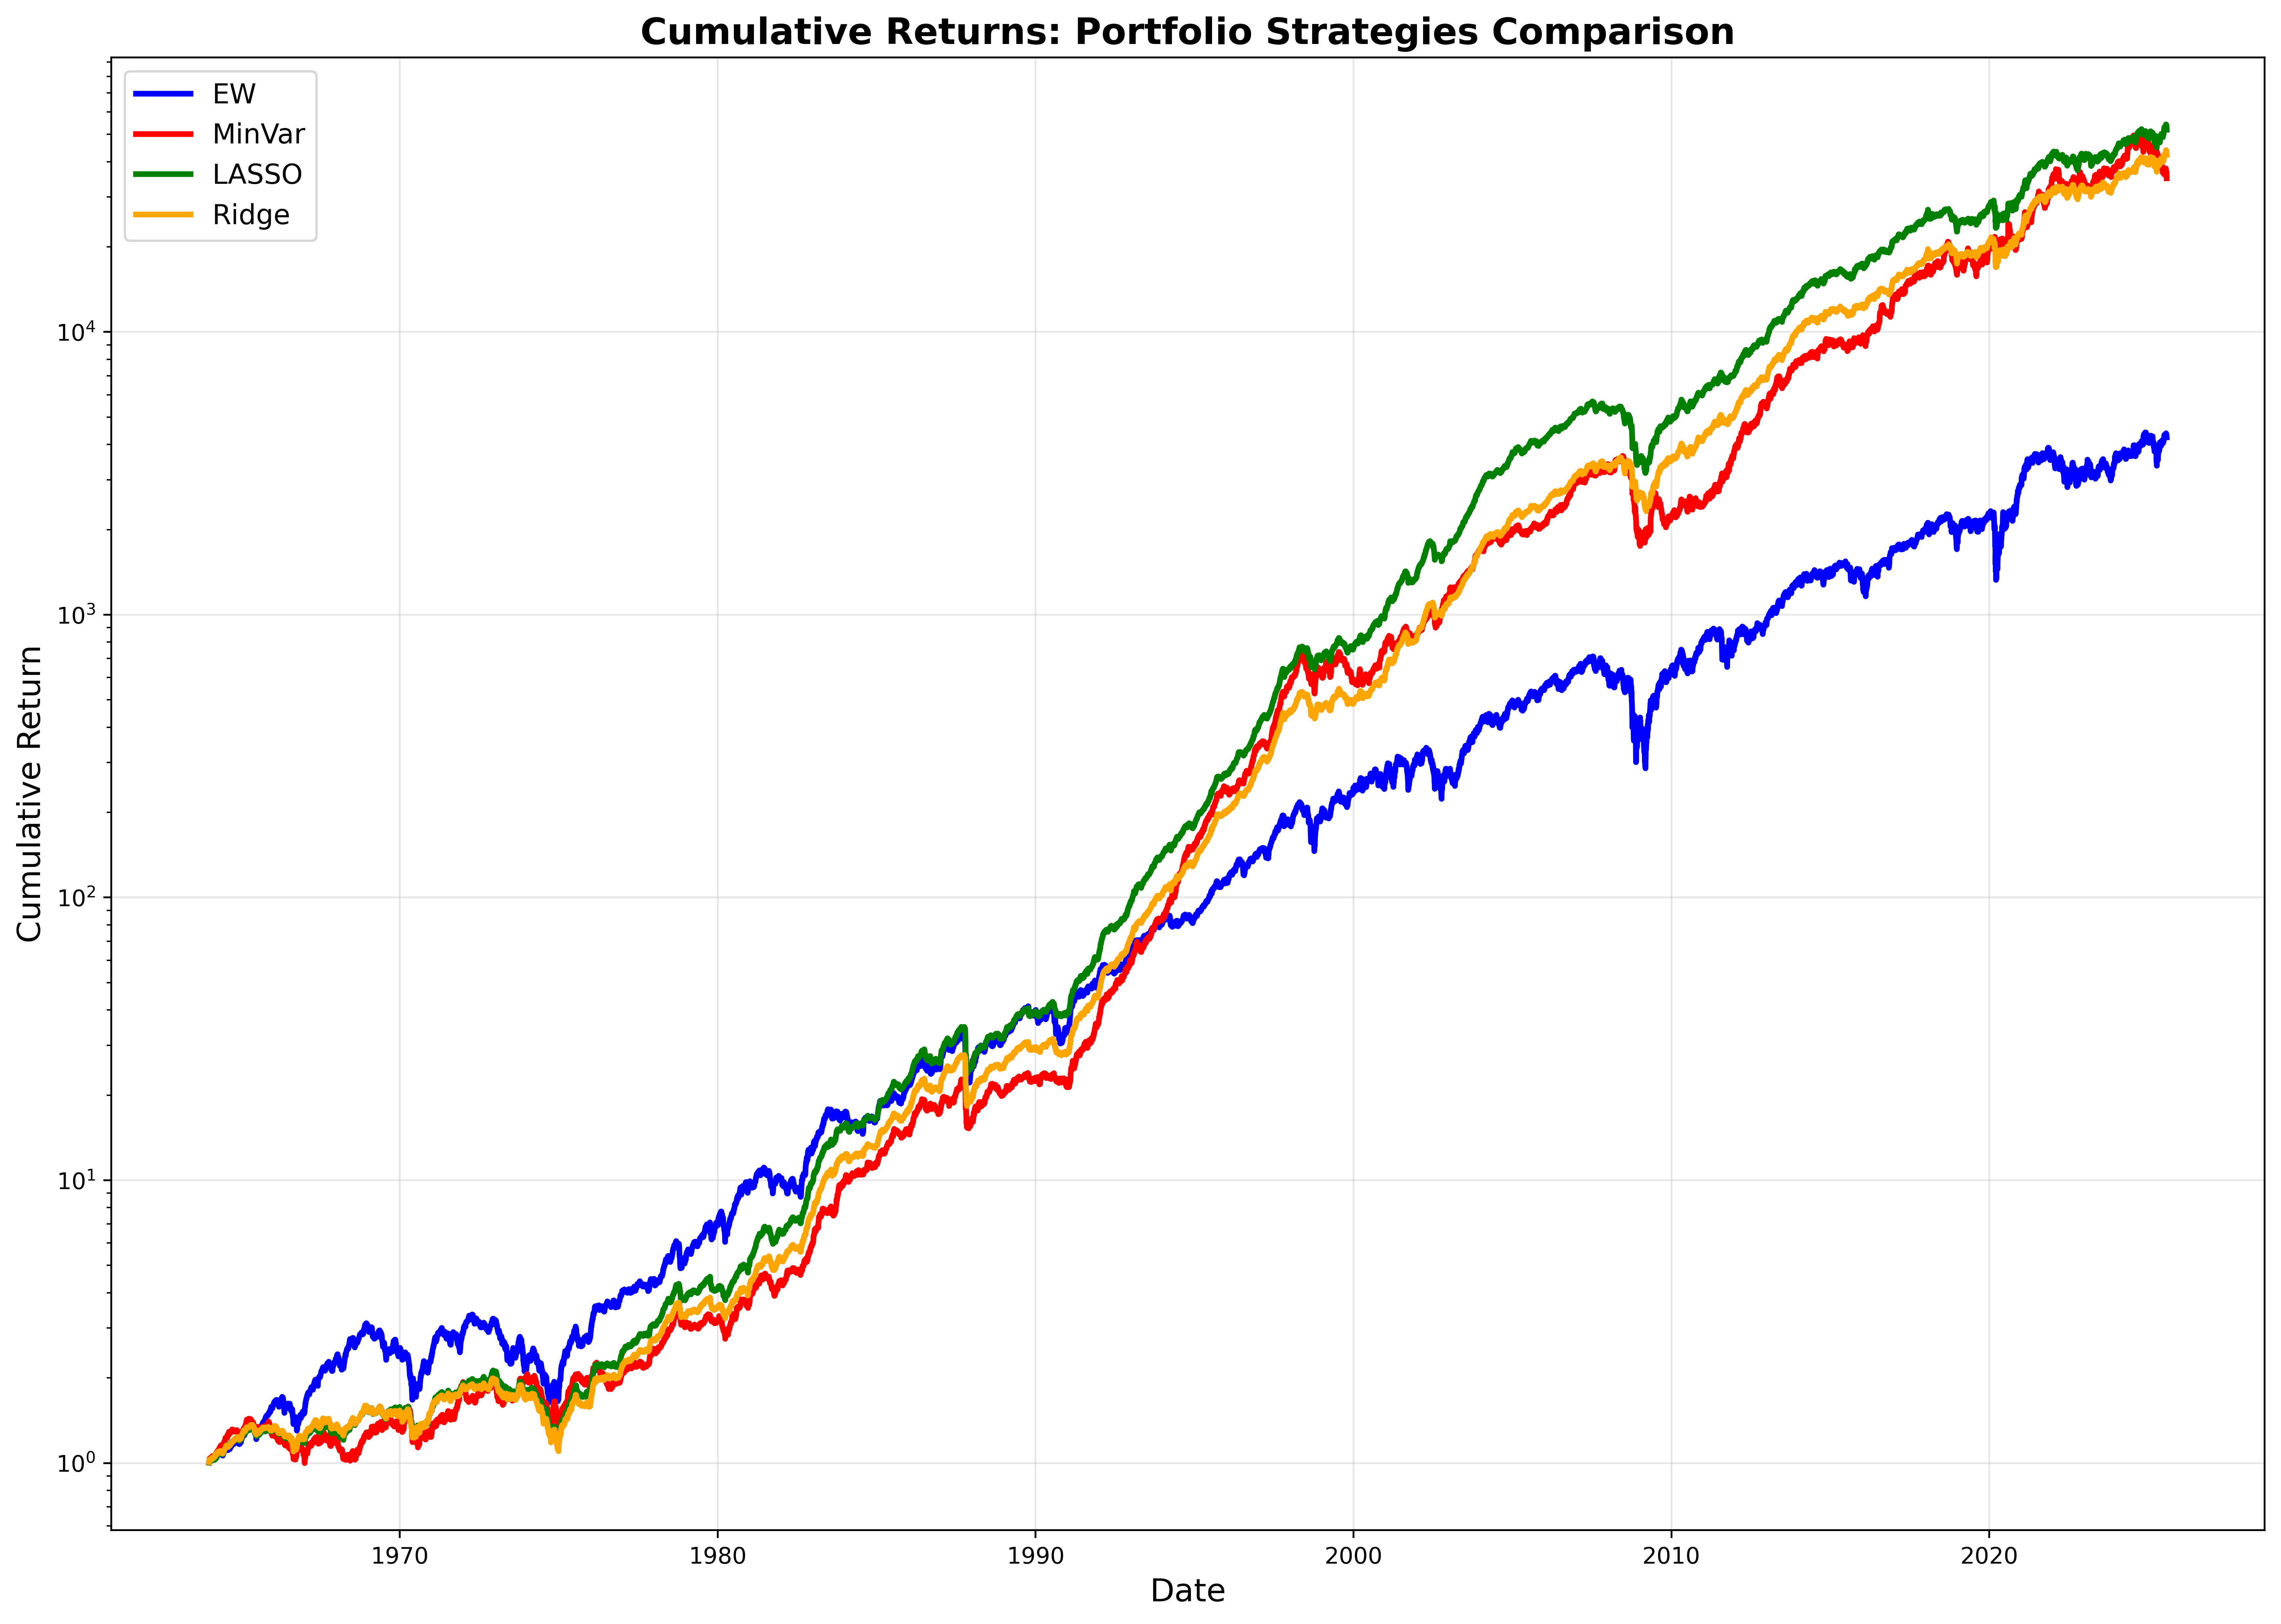
\includegraphics[width=0.5\textwidth]{figure1.png}
\caption{Cumulative Returns Comparison: Portfolio Strategies Performance. The chart shows the cumulative performance of four portfolio optimization strategies over the backtesting period. LASSO (green) and Ridge (orange) regularization methods significantly outperform both the Equal-Weighted benchmark (blue) and Minimum Variance approach (red), demonstrating the effectiveness of regularization in addressing overfitting issues in portfolio optimization.}
\label{fig:cumulative_returns}
\end{figure}

As illustrated in Table \ref{tab:performance} and Figure \ref{fig:cumulative_returns}, regularized approaches significantly outperform traditional methods.

\textbf{Key Findings from Validation Period:}
\begin{itemize}
    \item \textbf{LASSO best performer:} Sharpe ratio 0.0442, nearly triple equal-weighted benchmark
    \item \textbf{Ridge close second:} Sharpe ratio 0.0436 with lowest volatility (94.61\%)
    \item \textbf{Volatility reduction:} Both methods achieve 40\% lower volatility than equal-weighted (163.65\%)
    \item \textbf{Minimum variance fails:} Negative returns (-17.88\%) and Sharpe ratio (-0.1317), confirming overfitting
    \item \textbf{Benchmark validation:} Results match expectations (EW: 0.0165 vs 0.016, MinVar: -0.1317 vs -0.132)
\end{itemize}

\subsection{Regularization Path Analysis}
Optimal regularization parameters are automatically selected via \texttt{LassoCV} and \texttt{RidgeCV} as established in the course materials. The regularization paths reveal how penalty parameters balance the bias-variance tradeoff in the low signal-to-noise financial environment where 2\% $R^2$ represents strong predictive performance.


\section{Framework-Based Improvements and Extensions}

Building on the Data + Loss + Structure + Constraints framework, we identify improvements to enhance portfolio optimization beyond standard regularized approaches.

\subsection{Data Enhancements}

Manipulate the data input to improve signal quality and reduce noise.

\subsubsection{Increase Rolling Window Analysis}

Standard 126-day windows provide only 1.26 observations per feature for our 100-portfolio dataset, violating the rule of thumb requiring 5-10 observations per feature to avoid overfitting. Increasing window size to 252 days for more data points (2.52 observations per feature) should reduce overfitting and improve matrix conditioning. We compare both window sizes to evaluate this hypothesis.

\textbf{Theoretical Benefits:}
\begin{itemize}
    \item Larger sample size reduces covariance matrix estimation error
    \item 252-day window captures full seasonal patterns and market cycles
    \item Improved signal-to-noise ratio for all portfolio strategies
\end{itemize}

\textbf{Reproduction:}
To reproduce the 252-day window analysis results presented in Table \ref{tab:window_comparison}, run:
\begin{lstlisting}
python portfolio.py --mode 2
\end{lstlisting}

\textbf{Performance Comparison:}
Table \ref{tab:window_comparison} compares portfolio performance across different window sizes. The results validate our theoretical hypothesis: larger windows dramatically improve all portfolio strategies except for the EW strategy, with MinVar recovering from negative (-17.88\%) to positive (4.99\%) returns.

\begin{table}[h]
\centering
\caption{Window Size Impact on Portfolio Performance}
\label{tab:window_comparison}
\begin{tabular}{lcccc}
\hline
Strategy & Window & Daily Mean Return \(\%\) & Daily Volatility (\%) & Sharpe Ratio \\
\hline
EW & 126-day & 2.70 & 163.65 & 0.0165 \\
EW & 252-day & 2.70 & 163.65 & 0.0165 \\
MinVar & 126-day & -17.88 & 135.80 & -0.1317 \\
MinVar & 252-day & 4.99 & 93.95 & 0.0531 \\
LASSO & 126-day & 4.30 & 97.44 & 0.0442 \\
LASSO & 252-day & 6.96 & 93.14 & 0.0747 \\
Ridge & 126-day & 4.12 & 94.61 & 0.0436 \\
Ridge & 252-day & 7.27 & 90.80 & 0.0800 \\
\hline
\end{tabular}
\end{table}

\subsubsection{Portfolio Grouping for decreasing feature number}

Individual portfolio optimization suffers from insufficient data per feature, similar to how Meituan improved demand forecasting by using broader "fresh food" to predict specific "meat" subcategories. We group the 100 ME/OP portfolios into 9 logical categories to improve statistical reliability. Why 9? It is kind of a magic number that can make the rules of thumb work, but can be fine-tuned.

\textbf{Grouping Methodology}

We create a 3×3 matrix combining size and profitability dimensions. Size groups are Small (ME1-3), Medium (ME4-7), Large (ME8-10), while profitability groups are Low (OP1-3), Medium (OP4-7), High (OP8-10). Each group's return series is calculated as the equal-weighted average of its constituent portfolios, resulting in groups containing 9-16 portfolios each depending on the intersection size.

\textbf{Implementation}
\begin{itemize}
    \item Create 9 grouped return series by equal-weighting constituent portfolios
    \item Apply 4 Strategy as mentioned above to 9 groups (14 observations per feature)
    \item Distribute group weights equally among constituent portfolios
\end{itemize}

\textbf{Statistical Benefits:}
\begin{itemize}
    \item Improves from 1.26 to 14 observations per feature, avoiding overfitting problems
    \item Respects ME/OP factor structure while enhancing statistical reliability
    \item Reduces overfitting through logical dimensionality reduction
\end{itemize}

\textbf{Reproduction:}
To reproduce the portfolio grouping analysis results presented in Table \ref{tab:grouping_comparison}, run:
\begin{lstlisting}
python portfolio.py --mode 3
\end{lstlisting}

\textbf{Performance Comparison:}
Table \ref{tab:grouping_comparison} compares individual versus grouped portfolio optimization.

\begin{table}[h]
\centering
\caption{Individual vs. Grouped Portfolio Performance both with window size 126 days}
\label{tab:grouping_comparison}
\begin{tabular}{lcccc}
\hline
Strategy & Approach & Daily Return (\%) & Daily Vol (\%) & Sharpe Ratio \\
\hline
EW & Individual & 2.70 & 163.65 & 0.0165 \\
EW & Grouped & 2.70 & 163.65 & 0.0165 \\
MinVar & Individual & -17.88 & 135.80 & -0.1317 \\
MinVar & Grouped & 8.67 & 118.04 & 0.0735 \\
LASSO & Individual & 4.30 & 97.44 & 0.0442 \\
LASSO & Grouped & 8.46 & 119.13 & 0.0710 \\
Ridge & Individual & 4.12 & 94.61 & 0.0436 \\
Ridge & Grouped & 7.71 & 116.88 & 0.0660 \\
\hline
\end{tabular}
\end{table}

\textbf{Key Findings from Portfolio Grouping Analysis:}

The empirical results strongly validate our theoretical hypothesis about reducing overfitting through improved observations-per-feature ratios. The portfolio grouping approach demonstrates several critical insights:

\begin{itemize}
    \item \textbf{MinVar Overfitting Resolution:} MinVar recovers from negative returns (-17.88\%) to positive (8.67\%), with Sharpe ratio improving from -0.1317 to 0.0735
    \item \textbf{EW Unchanged:} Equal-weighted remains identical (0.0165 Sharpe) as expected
    \item \textbf{Regularization Improvement:} LASSO (0.0442 to 0.0710) and Ridge (0.0436 to 0.0660) both show higher Sharpe ratios
    \item \textbf{Statistical Validation:} 14.0 vs 1.26 observations per feature successfully addresses overfitting
\end{itemize}

The results demonstrate that portfolio grouping effectively balances the bias-variance tradeoff by reducing estimation error at the cost of some model complexity, making it particularly valuable for traditional optimization approaches that lack inherent regularization mechanisms.

\subsection{Dynamic Constraints for Regime-Adaptive Portfolios}

\subsubsection{Empirical Motivation}
Analysis of cumulative returns in Figure \ref{fig:cumulative_returns} reveals optimal regime-dependent strategy selection: LASSO regularization excels during high volatility periods by filtering out unreliable assets through feature selection, while equal-weighted portfolios provide robust performance during stable low volatility environments. This pattern suggests adaptive strategy selection based on market volatility levels.

\subsubsection{Mathematical Framework and Implementation}
\textbf{Adaptive Strategy Selection Framework:}
\begin{align}
Strategy_t = \begin{cases}
\text{LASSO} & \text{if } \hat{\sigma}_{mkt,t} > \mu_{\sigma} + 0.5\sigma_{\sigma} \\
\text{Equal Weight} & \text{if } \hat{\sigma}_{mkt,t} \leq \mu_{\sigma} + 0.5\sigma_{\sigma}
\end{cases}
\end{align}
where $\hat{\sigma}_{mkt,t}$ is rolling 126-day market volatility, $\mu_{\sigma}$ is historical average volatility (5 years), and $\sigma_{\sigma}$ is volatility of volatility. This idea is similar to the mix decision tree + leaves being linear regression. depends on the regime, use different strategy.

\textbf{Reproduction:}
To reproduce the regime-adaptive strategy results, run:
\begin{lstlisting}
python portfolio.py --mode 4
\end{lstlisting}

\subsubsection{Performance Comparison}
This method performs less good than expected, possibly due to the simplistic thresholding approach and limited regime differentiation. More sophisticated regime detection and strategy blending could yield better results.

\section{Conclusion}

This study demonstrates that regularization techniques effectively address the bias-variance tradeoff in portfolio optimization. While minimum variance portfolios suffer from overfitting with extreme weights, LASSO and Ridge regularization provide superior out-of-sample performance through automatic feature selection and coefficient shrinkage.

Data transformation techniques are also beneficial to solve overfitting problems and often prove highly effective. Portfolio grouping demonstrates significant improvements, with MinVar recovering from negative (-0.1317) to strong positive performance (0.0735 Sharpe), while LASSO (0.0710) and Ridge (0.0660) also show enhanced results. Extended 252-day windows improve all strategies by providing better statistical foundations.

We may also combine the mentioned improvements together to further enhance performance. Due to limited time, we didn't try out this idea, but it is worth exploring in future work.

\textbf{Key Takeaway:} Often, the most impactful improvements come from thoughtful data manipulation rather than solely relying on complex modeling techniques. Both regularization and strategic data transformations improved portfolio optimization in our study.

\end{document}